
\subsection{Measuring functional distance using an NMF filter}

Based on the clear patterns in Figure \ref{H}, we hypothesized that NMF-filtered Pfam distance would be a useful metric for functional distance between sites. To test this idea, we compared how well different measures of functional distance were modeled by a combination of environmental distance and geographic distances in a naive regression model.  Using adjusted $R^2$ as a measure of overall correlation, we found that the correlation of NMF-filtered Pfam distance with environmental and geographic distances (overall adjusted $R^2 = 0.24$) was comparable to that of unfiltered Pfam distance (adjusted $R^2 = 0.25$), and higher than that of PCA-filtered Pfam distance using the same number of components (adjusted $R^2 = 0.15$). This suggests that the NMF filtering retains more information relevant to these correlations than PCA filtering.

Therefore, we used NMF-filtered Pfam distance to ask about patterns across sites. Specifically, how did functional distance between sites correlate with environmental and geographic distance?  Environmental distances were calculated as Euclidean distances of normalized environmental variables (see Materials and Methods), while geographic distances were calculated using great circles. We used logged geographic distances as our main predictor so as not to give too much emphasis to large distances in our linear models.

We found that our measure of functional distance was more correlated with overall environmental distance (Figure \ref{scatter5}a) than with logged geographic distance (Figure \ref{scatter5}b). We confirmed this result with a multivariate Mantel test; when both distances were used as predictors, the partial correlation between Pfam distance and environmental distance ($\rho=0.45$, $P < 0.001$) was much higher than that between Pfam distance and logged geographic distance ($\rho=0.11$, $P=0.02$). This result was similar to that found by \cite{RaesLetu11}, although our partial correlation for environmental distance was substantially higher (0.45 vs. 0.27).  Although it was also statistically significant, the partial correlation with geographic distance (0.11) seems so low as to be biologically negligible. These results were robust to different choices of ranks in the NMF decomposition (Figure \ref{NMF_fig4}).

\begin{figure}
\centering
%\subfigure[]{\includegraphics[width=2.4in,height=2.4in]{GOS/scatter5.Rout-0.pdf}}
%\subfigure[]{\includegraphics[width=2.4in,height=2.4in]{GOS/scatter5.Rout-1.pdf}}
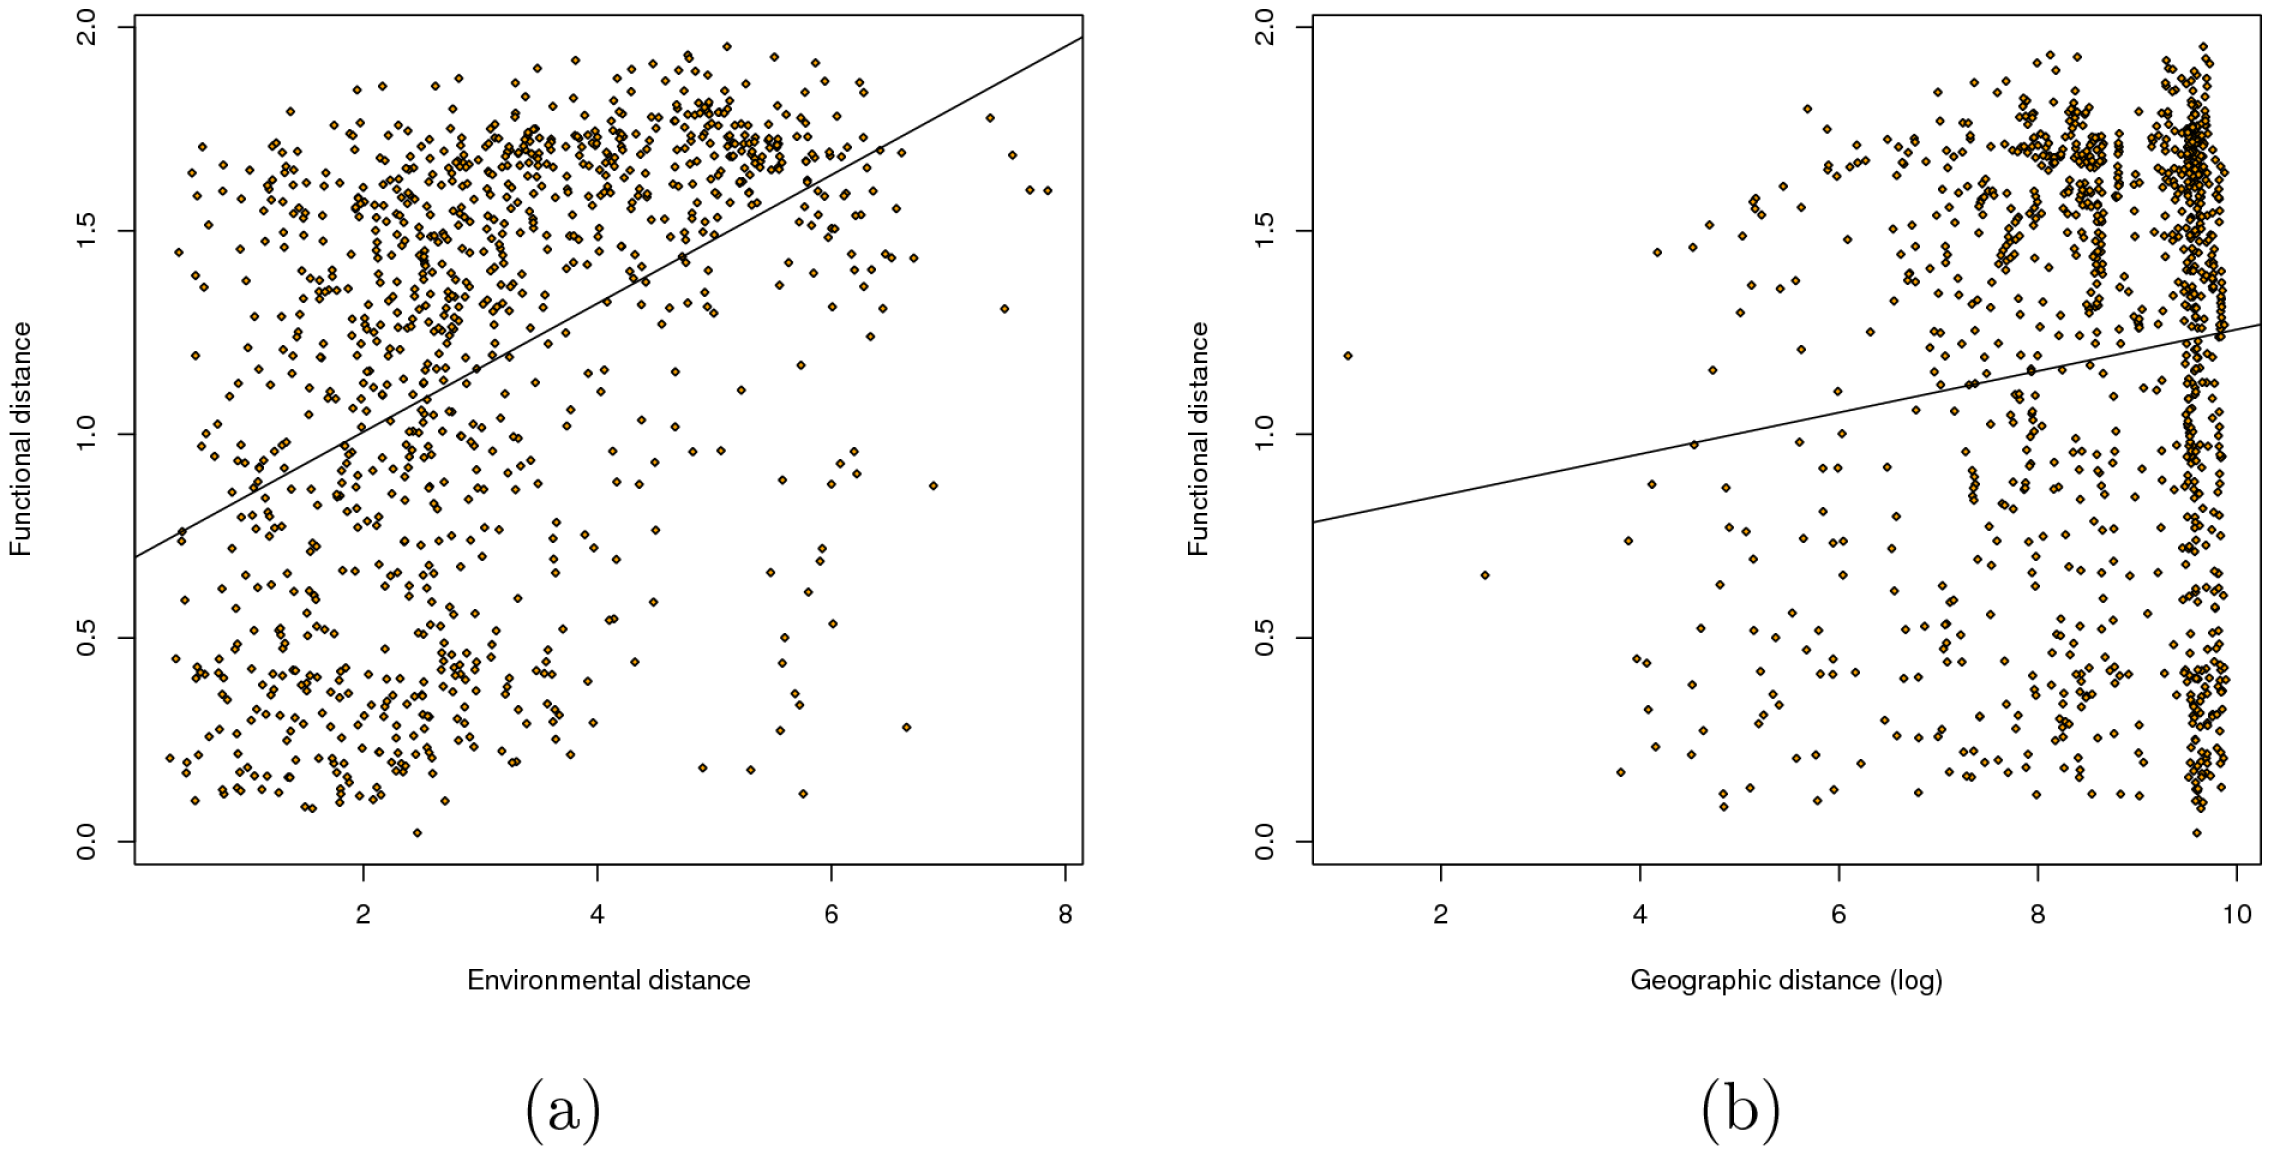
\includegraphics[width=\textwidth]{NMF/figures/fig4}
\caption{\textbf{Pairwise correlation between distances. } a. Environmental distance vs. functional distance (cor=0.451, P $<$0.001, regular Mantel test).  b. Logged geographic distance vs. functional distance (cor=0.127, P=0.014).}
\label{NMF_fig4}
\end{figure}

Next, we superimposed the Pfam similarity matrix $S$ on a global map to visualize how functional differences were influenced by environmental conditions and geographic location (see \ref{global}).  In the global map we connected sites based on their functional similarity and their environmental similarity respectively.  The number of lines connecting sites depended on an arbitrary choice of similarity threshold.  A movie showing how this pattern changes over a wide range of thresholds is available as Movie S1.  Many early links were established between sites that were well-separated geographically, consistent with our result that the Pfam similarity of microbial communities was more strongly associated with environmental differences than with physical distance.  

\begin{figure}
\label{global}
\centering
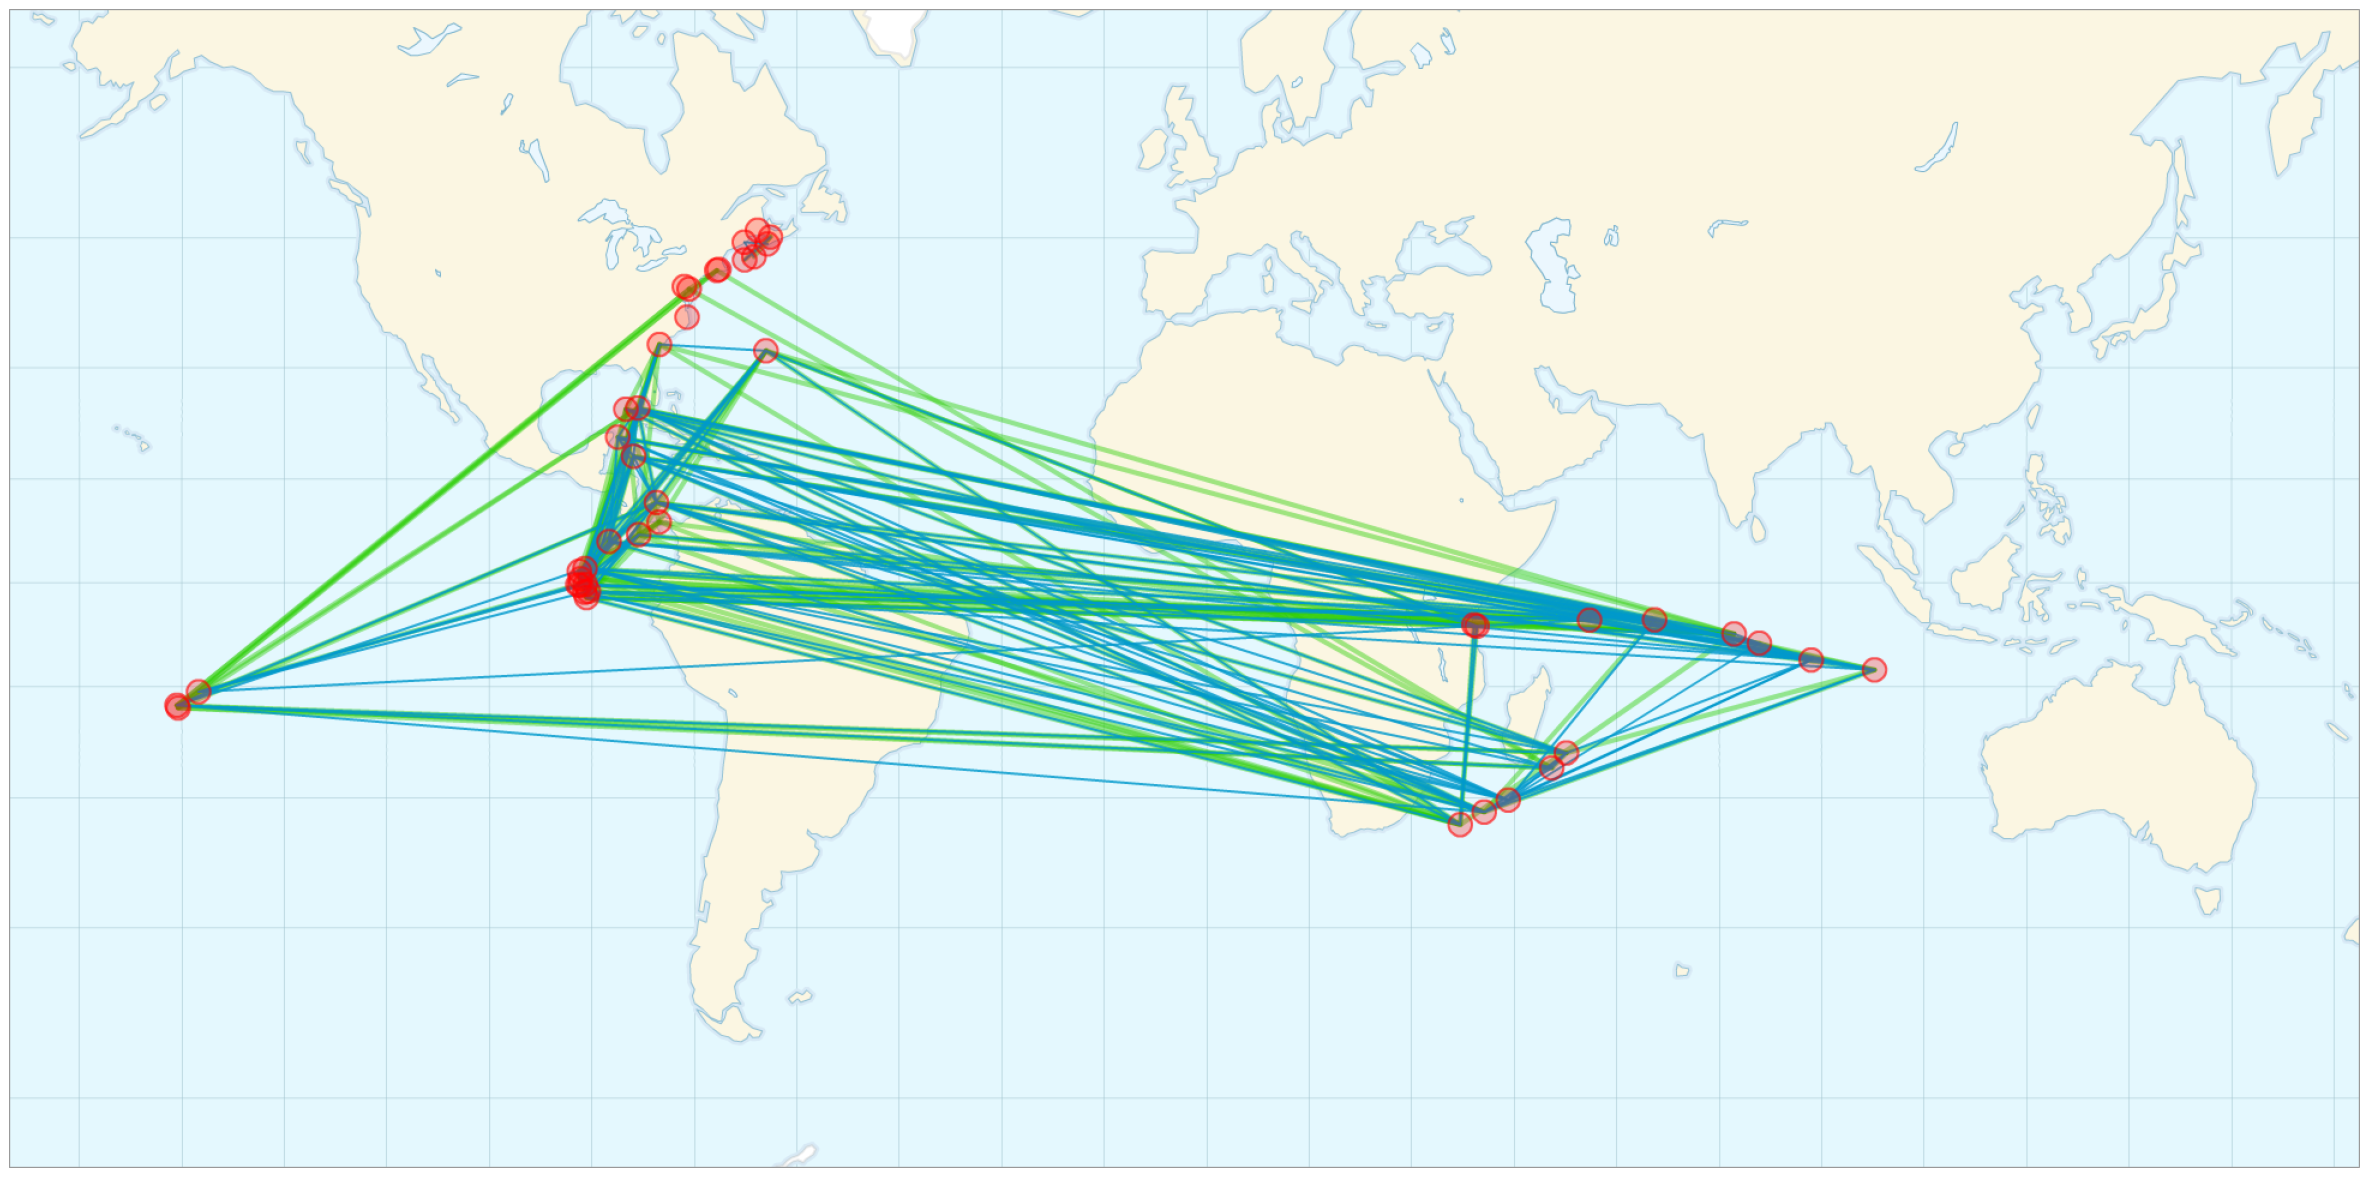
\includegraphics[width=\textwidth]{NMF/figures/fig5}
\caption[]{\textbf{Functional and environmental similarity on a global map. } The 120 pairs of sites with highest functional (environmental) similarity are linked in blue (green).  Environmental similarity is calculated from the environmental distance matrix $D$ using the transformation $1/(1+D)$. A movie showing this pattern over a range of similarity thresholds is available as Movie S1.}
\label{NMF_fig5}
\end{figure}

